\begin{mainquestion}{reverse_protection}{Reverse Polarity Protection}

Alexander has been having a terrible, horrible, no good, very bad day. He's rebuilt his circuit twice after accidentally connecting his power supply backwards (D'oh!). But no more! Let's build a reverse protection circuit and stop these headaches.

Alexander's first idea was to use a diode to prevent reverse current. Consider the circuit below:

\begin{center}
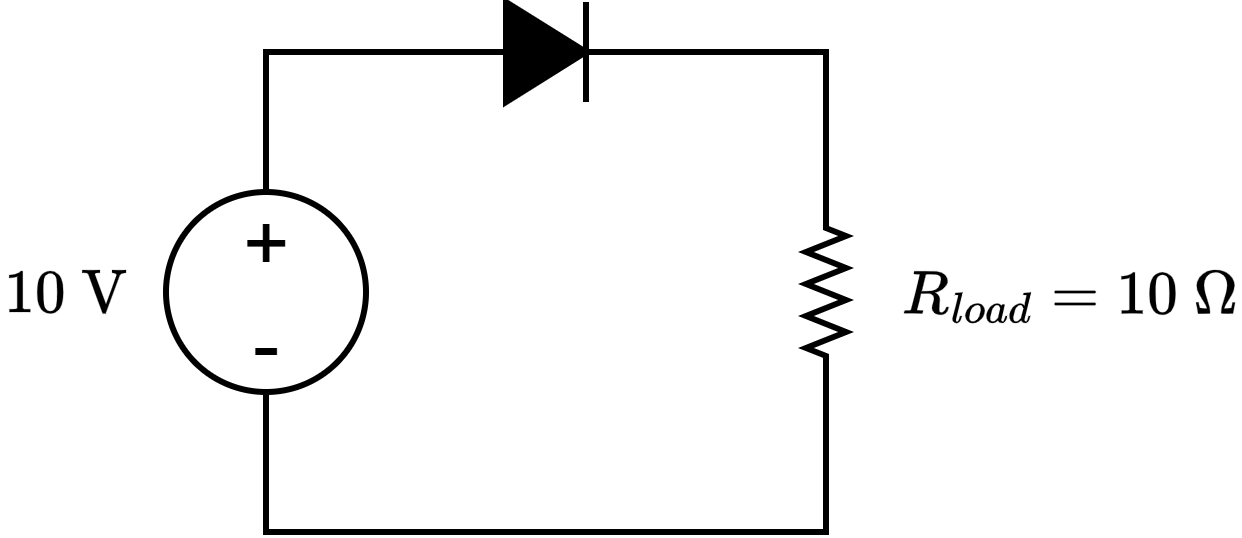
\includegraphics[height=1.4in]{diode.png}
\end{center}

\begin{partquestion}{diode_eff}{Using a constant-voltage drop model of \qty{0.7}{\volt}, find the power delivered to $R_{load}$ and the power delivered to the diode. What is the efficiency of this circuit?}

\begin{answer}
    Assuming the diode drops \qty{0.7}{\volt}, the voltage across $R_{load} = 10 - 0.7 = \qty{9.3}{\volt}$. The current can be found using Ohm's law, as $\qty{9.3}{\volt} / \qty{10}{\ohm} = \qty{0.93}{\ampere}$. Now that we have all the voltages we can find the power in the load:
    \[
    P(R_{load}) = \qty{9.3}{\volt} \cdot \qty{0.93}{\ampere} = \qty{8.65}{\watt}
    \]
    And the power in the diode:
    \[
    P(D) = \qty{0.7}{\volt} \cdot \qty{0.93}{\ampere} = \qty{651}{\milli\watt}
    \]
    Which sets the efficiency as:
    \[
    \eta = \frac{8.65}{8.65 + 0.651} = 0.93 \rightarrow 93\%
    \]
\end{answer}
\end{partquestion}

Alexander's mentor came by and recommended he instead try a MOSFET protection circuit and sketched the following:

\begin{center}
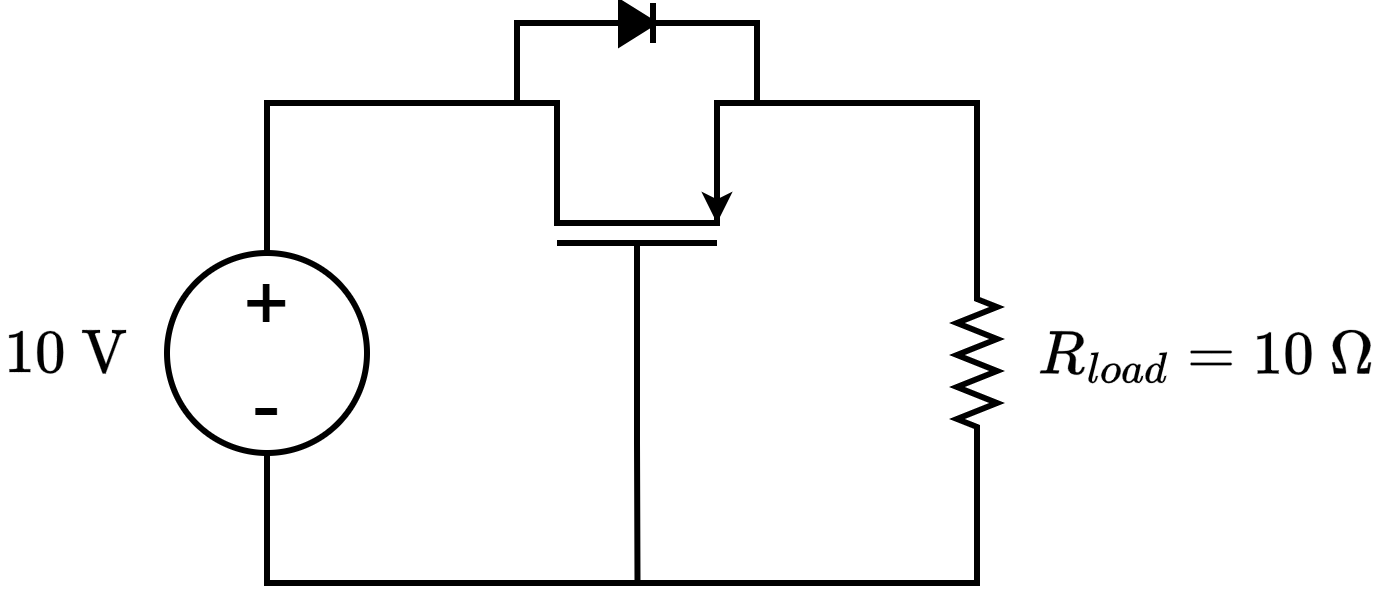
\includegraphics[height=1.4in]{pmos.png}
\end{center}

\begin{partquestion}{pmos}{In what region is this PMOS operating? What about in reverse polarity (flipping the voltage source backwards)?}
\begin{answer}
    Assuming the diode is conducting as before, we would assume $V_S$ to be near \qty{9.3}{\volt}. In this situation, we now have $V_{SG} = \qty{9.3}{\volt}$ and $V_{DS} = \qty{0.7}{\volt}$. Since for all reasonable threshold voltages $V_{SG} - V_T > V_{DS}$, we can agree the PMOS should be operating in the linear region. Even if the diode was suddenly removed, the extremely high $V_{OV}$ would open the channel wide enough to support the current.

    With the supply polarity reversed, now the diode would be off. If we assume the PMOS also blocks current, then $V_{S} = 0$ by Ohm's law, so $V_{SG} = 0$. This comfortably places the PMOS in the cutoff regime so no current flows.
\end{answer}
\end{partquestion}

\begin{partquestion}{datasheet}{You have a \href{https://www.vishay.com/docs/91076/91076.pdf}{IRF9530} power PMOS device. Find estimates for the transconductance $k_n$ and threshold voltage $V_{th}$ from the datasheet.}
\end{partquestion}

\begin{partquestion}{pmos_eff}{Find the total power delivered to the $R_{load}$ and the PMOS in forward polarity. What's the efficiency of this circuit? Use the drain current equation in the linear region using your estimates from part (\cref{prob:reverse_protection:datasheet}) for $k_n$ and $V_{th}$}
\end{partquestion}

\begin{partquestion}{rds}{The datasheet also mentions that the PMOS has an "on resistance" of \qty{0.3}{\ohm}. Repeat (\cref{prob:reverse_protection:pmos_eff}) but simplify the PMOS model to be just a resistor. How accurate is this approximation?}
\end{partquestion}

\begin{partquestion}{comp}{Invent a complementary version of this circuit that protects a negative supply from reverse polarity.}
\end{partquestion}

\end{mainquestion}
